\subsection{Design Concepts}

Our goal is to enter text in VR conveniently, accurately, and quickly using existing VR controllers, without a steep learning curve.  Our initial investigation informs us that users find it difficult to hit the right key because of the lack of proprioception, and swiping, though better than tapping, is still slow because of the visual latency.  O

Our design is centered around three main concepts: relative positioning, directional swiping, and mixed keyboard modes, as explained below. 

\begin{comment}

Our design efforts focused on balancing three of the above factors: input speed, learning time, and physical size.
Our thinking was particularly influenced by the interaction design of cell phones that use T9 input, which relies on a database of words to disambiguate cell phone keypad keystrokes that are associated with more than one letter.
If we could design an input device that combined the best of the standard keyboard (fast text input, familiar layout) and the 12-key cell phone keypad (small size), we would have a device that could be used in off-the-desktop situations, potentially for extended typing tasks, with little degradation in performance. 

Despite the difficulties for the users to physically locate their finger outside of the virtual environment in order to interact with the keyboard on a mobile phone, the users are not completely helpless from their previous typing experience.
To start with, the users have muscle memory from typing on traditional mobile keyboards. With this previous experience, the user remembers, although imprecise, the location of letters if the layout of the keyboard is the same as what they are used to.

Thus, to leverage these previous knowledge of the users and address the problem that the users cannot physically see their fingers, we center our designs around two key features that we believe can help them adjust to typing in virtual reality: relative finger tracking, and batched keys.

Traditional mobile keyboard requires users to tap on the key precisely to enter an individual letter.
This method falls prey to specifically to the problem described above: users cannot tap on the individual keys accurate enough because they cannot see their finger relative to the touch screen of the mobile phone in a virtual environment.
Thus, 
\end{comment}

\subsection{Directional Vectors as Key Entries}

The goal of our first design concept is to minimize the need for visual feedback and to  
compensate for the lack of proprioception.  The idea is to use relative positioning, rather than asking the users to hit absolute positions on the invisible keyboard. Relative movement, instead of absolute movements, have also been found to be beneficial in reducing fatigue~\cite{Hincapie-Ramos:2014:CEM:2556288.2557130} so the user can start the interaction from their current position. 

We lay out keys of our virtual keyboard exactly as the original keyboard.  Typing a letter involves touching the keyboard, dragging and removing the finger.  The first touch is assumed to hit the centroid of the keyboard, which is the position right between the F and the G keys, independent of where the finger touches the touchpad.  The user then drags the finger to the position of the key of interest.  A trail showing the path of the finger is shown.   This takes advantage of the user’s familiarity of the keyboard.  

This approach based on relative positioning is different from swiping in several important ways. 
\begin{enumerate}
\item
In the case of swiping, the user has to decide how to hit the first letter correctly.  Here the entry of the first letter is the same as for all subsequent letters.  The first touch defines the center of the keyboard, and the user drags it to the right key for each character.   
\item
With swiping, the finger connects between each pair of consecutive letters.  In our case, the user connects the centroid to each key.   Since the users are familiar with the layout of the original keyboard, users can determine the directional vector from the centroid easier than figuring out the vectors between each pair of keys. 
\item 
With swiping, the worst-case distance traveled for each letter could be the length of the keyboard.  In our case, the worst-case is half the width of the keyboard. 
\end{enumerate}

\subsection{Directions as Key Entries}

With direction vectors, the time it takes to enter a key is proportional to the distance from the centroid.  Furthermore, the user has to make sure that he has to stop at the right key in each direction.  We optimize the input method further by asking the users to just get the directions right, and rely on error correction techniques to determine the intended word.  Most users are familiar with online error correction on mobile text input. 

We quantize the directions into just 6 intervals: top left, top right, left, right, bottom left, and bottom right.   In another words, the user can think of the keyboard having six tiles: with two tiles representing the left and right halves of each of the three bottom rows.  The user needs only to drag his finger to the appropriate tile.  The layout of the tiles is shown in Figure~\ref{fig:swipeVRLayout}.

\begin{figure}
  \centering

%  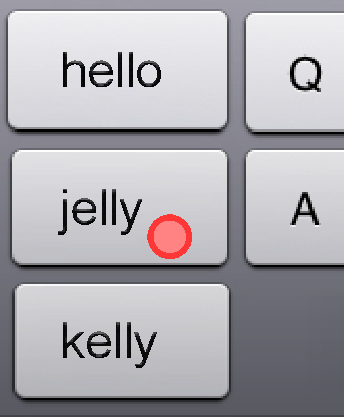
\includegraphics[width=.3\columnwidth]{figures/multiword}
  
  \caption{The six tiles of the direction-based keyboard.}
  ~\label{fig:swipeVRLayout}
\end{figure}

If the letters typed can correspond to multiple words, then the user is offered a choice, starting with the most frequently occurring words.  The user simply has to drag his finger to the intended word. 

This proposal has the advantage that users only have to indicate the direction: the vectors dragged are short for all letters.  The inputs can therefore take a short, constant time, regardless of the distance of the key from the centroid.  It is also relatively easy for users to indicate one of six directions accurately, without visual feedback.  The downside is that there may be a need of error correction due to ambiguous inputs.  By analyzing the dictionary, we found AMBIGUOUS-WORD-RESULTS.

We use a Bayesian word recommender to infer the most probable words among words that correspond to the same tile sequence.  For example, the words ``hello" and ``jelly" has the same representation.  
This recommender algorithm use 2-gram and 3-gram data from Google Books Ngram Viewer\footnote{http://storage.googleapis.com/books/ngrams/books/datasetsv2.html}, part of speech frequency for English dictionary, individual word frequency for the entire English language, and produces a prediction score.
The word with highest prediction score will be selected as the most probable word.

Characters are not displayed one at a time, but rather the whole word appears all at once, and sometimes with a choice for users to select from, as shown in Figure~\ref{fig:multiword}.


\begin{figure}
  \centering

  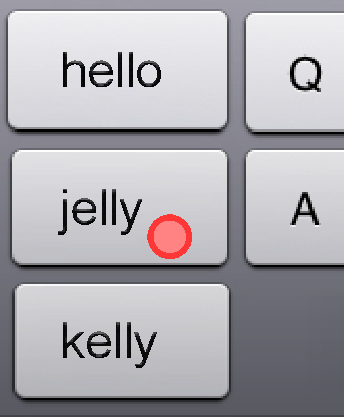
\includegraphics[width=.3\columnwidth]{figures/multiword}
  
  \caption{Users are presented with words represented by the same sequence of tile inputs.}
  ~\label{fig:multiword}
\end{figure}

\subsection{Hybrid Keyboards}

While the directional inputs are much faster, but users may wish to type in words not in the dictionary.  Common examples are user names or password entries.  The user also may have to enter numbers, punctuations, special keys etc. 

Our design is to adopt a hybrid keyboard.  Since our optimized “direction-only” keyboard has the same key layout as the original keyboard, we can present a consistent view to the user and let the user switch modes between these two.  

The keyboard switching is implicitly based on the intention of the user.  As the user slows down to hit the specific key, our keyboard automatically infers that the user wishes to control the text entry at the key level. 

In addition, we introduce a few shortcuts for the “delete” and the “space” keys.   Users can double tap the touch screen to indicate delete.  For the space key, the user can click a specific physical button on the controller, such as the “trigger” button on the bottom side of the Vive controller.  We have also experimented automatically inserting a space after a certain timeout period between 150 and 500 ms.  However, we found that users preferred to have the control of when to insert the space themselves.   

\begin{figure*}
  \centering
  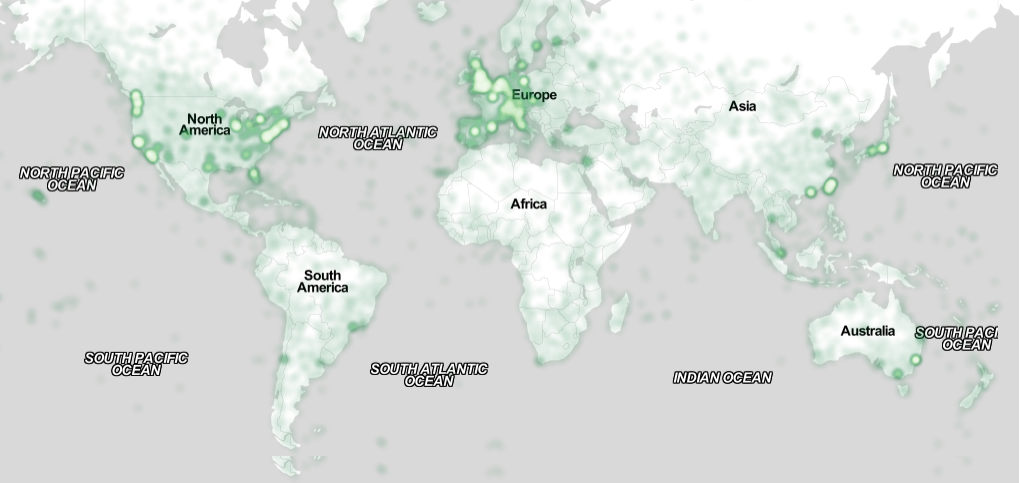
\includegraphics[width=1.75\columnwidth]{figures/map}
  \caption{Example of the system.  When the user want to type .}
  ~\label{fig:example}
\end{figure*}

\begin{figure}
\centering

  \begin{tikzpicture}

  \def \n {5}
  \def \radius {3cm}
  \def \margin {8} % margin in angles, depends on the radius

  \foreach \s in {1,...,\n}
  {
    \node[draw, circle] at ({360/\n * (\s - 1)}:\radius) {$\s$};
    \draw[->, >=latex] ({360/\n * (\s - 1)+\margin}:\radius) 
      arc ({360/\n * (\s - 1)+\margin}:{360/\n * (\s)-\margin}:\radius);
  	}
	\end{tikzpicture}

	\caption{
    Controller\\
	Intent Detection Classifier\\
    triager \\
	|swipe          |                |\\
    ngram           deterministic     \\
    selection        letter           \\
}~\label{fig:systemFlowchart}
\end{figure}

\subsection{Informal Evaluation of Alternative Design Choices}

Our informal evaluation of this proposed text entry indicated that it is significantly better than any of the methods described in the last section.   To arrive at this proposal, we have tried out many different combinations, all of which have decisively weaker performances.  The combinations we tried include: 

\begin{enumerate}
\item
Six-tile design and tapping with absolute positioning.  The mobile keyboard is divided into the six times, the user only needs to only tap on the right tile, relying on error correction to find the right word.   We found the error rate of this input method to be too high, because users cannot hit the six tiles accurately enough. 

\item
Six-tile design and swiping with absolute positioning.  This design is faster that swiping on a 26-key keyboard, but it is still too slow.  HOW MUCH SLOWER.

\item 
Eight-tile design with two cursors and relatively positioning.  Since most people type with two hands on the keyboard, we experimented introducing two cursors into the proposed design.  We split the keyboard into the left and right half, and the initial positions of the left and right thumbs are assumed to be the centroid of each half.  Instead of having 6 directions for each hand, we simplify it to four directions each (up, down, left,  right).  This can also reduces the number of ambiguous entries. 

Our informal evaluation of this method quickly pointed out the flaw of this design.  It was too complicated, as the user has to decide which hand to move, and then which of the four directions.  Furthermore, we found that with the one virtual cursor design, the user usually uses the other hand to enter the special but common “delete” and “space” keys etc. 
\end{enumerate}

Because none of the choices come close to the proposed entry method, our evaluation focuses primarily on understanding the characteristics of that technique. 

